\chapter{Research Topic 1}
\label{cha:research_topic_1}

Equation \ref{eq:example} is an example equation that is relatively famous in physics \cite{einstein_ist_1905}. 
\begin{equation}
    \label{eq:example}
    E = m c^2
\end{equation}
One could discuss this equation in more details in appendix \ref{app:long_proof} but that is outside the scope of this template thesis. 
An example figure can be inserted as shown by figure \ref{fig:example_figure}
\begin{figure}[!htb]
    \centering
    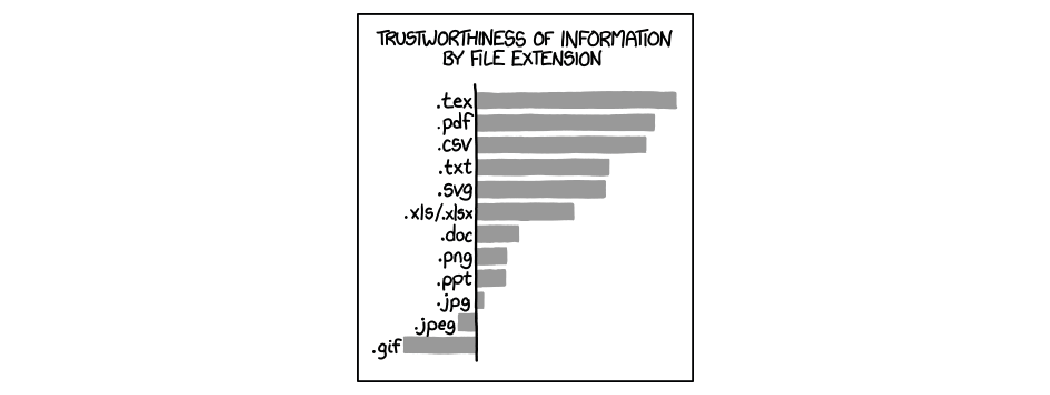
\includegraphics[width=1\textwidth]{example_figure.pdf}
    \caption[Short version of caption for list of figures comes first in brackets.]{
    Short version of caption for list of figures comes first in square brackets. The complete caption comes that comes in the curly brackets can be much longer but we don't want all of that caption to be included in the list of figures. 
    The example figure is from \url{https://xkcd.com/1301/}.
    }
    \label{fig:example_figure}
\end{figure}
Notice that equation numbers, figure numbers, chapter numbers and citations are all clickable in the PDF (thanks to hyperref), which makes a world of difference for documents that are mostly going to be used digitally.

\paragraph{}
\Blindtext[2]
